\chapter{Fejlesztői dokumentáció}
\label{ch:impl}

\section{Megoldási terv}

\subsection{Követelményelemzés}

A weboldal használatakor négy típusú felhasználó különböztethető meg: vendég, bejelentkezett felhasználó, moderátor és adminisztrátor. Az előző fejezethez hasonlóan, itt is ezek alapján történik meg a funkcionális követelmények definiálása.

\subsubsection{Vendég}
\begin{compactitem}
	\item Térkép megtekintése:
		\begin{compactitem}
			\item Alapvető irányítási lehetőségek: mozgatás, forgatás, nagyítás/kicsinyítés
			\item Az összes pont helyzetének megfelelő megjelenítése, fontosabb információk jelölésével
			\item Pontra kattintáskor sorszám, kép és megjegyzés megtekintése, hivatkozás annak adatlapjára
		\end{compactitem}
	\item Pont részletezése:
		\begin{compactitem}
			\item Minden információ megjelenítése
			\item Közvetlen hivatkozások a feltöltő profiljára, a térképen való megtekintésre és az adatlap megtekintésére
		\end{compactitem}
	\item Pontok listázása:
		\begin{compactitem}
			\item Pontok közötti szűrés, lapméret állítása
			\item Fontosabb információk megjelenítése
			\item Közvetlen hivatkozások a feltöltő profiljára, a térképen való megtekintésre és az adatlap megtekintésére
		\end{compactitem}
	\item Színséma választása:
		\begin{compactitem}
			\item Sötét és világos mód közötti váltás bárhol 
		\end{compactitem}
	\item Regisztráció:
	\begin{compactitem}
		\item Felhasználónév megadása
		\item E-mail cím megadása
		\item Jelszó megadása és megerősítése
		\item Profilkép megadása
		\item Regisztráció gombra nyomva:
		\begin{compactitem}
			\item siker esetén: automatikus bejelentkeztetés az új fiókba
			\item sikertelenség esetén (hiányzik egy kötelező adat, vagy felhasználónév/e-mail cím már foglalt): hibaüzenet megjelenítése a sikertelenség okával feltüntetve
		\end{compactitem}
	\end{compactitem}
	\item Bejelentkezés:
	\begin{compactitem}
		\item Felhasználónév megadása
		\item Jelszó megadása
		\item Bejelentkezés gombra nyomva:
		\begin{compactitem}
			\item siker esetén: bejelentkeztetés a fiókba
			\item sikertelenség esetén (hiányzik egy adat, vagy felhasználó-jelszó páros nem megfelelő): hibaüzenet megjelenítése a sikertelenség okát NEM feltüntetve
		\end{compactitem}
	\end{compactitem}
\end{compactitem}

\subsubsection{Bejelentkezett felhasználó}
\begin{compactitem}
	\item Minden, amit egy vendég is tud (értelemszerűen a regisztráció és bejelentkezés kivételével)
	\item Kijelentkezés:
	\begin{compactitem}
		\item Kijelentkezés gombra kattintva kijelentkezteti a felhasználót és elnavigálja a kezdőoldalra
	\end{compactitem}
	\item Új pont bejelentése:
	\begin{compactitem}
		\item Koordináták (kötelező) megadása, saját koordináták automatikus meghatározása
		\item Település és -rész megadása
		\item Méret megadása
		\item Hozzáférhetőség megadása
		\item Szemét típusának megadása
		\item Opcionális megjegyzés megadása
		\item Képek hozzáadása
		\item Bejelentés gombra nyomva:
		\begin{compactitem}
			\item siker esetén: pont létrehozása és elnavigálás az előzőleg látogatott aloldalra
			\item sikertelenség esetén (hiányzó koordináták, érvénytelen adatok megadása): hibaüzenet megjelenítése a sikertelenség okát feltüntetve
		\end{compactitem}
	\end{compactitem}
	\item Pont szerkesztése:
	\begin{compactitem}
		\item Minden bejelentéskor megadott adat frissítése
		\item Új állapot megadása
		\item Módosítás gombra nyomva: hasonló funkcionalitás a bejelentésekor kattintott Bejelentés gomb esetén
	\end{compactitem}
	\item Saját profil megtekintése:
	\begin{compactitem}
		\item Profilkép megjelenítése
		\item Felhasználónév megjelenítése
		\item E-mail cím megjelenítése
		\item Hivatkozás saját profil szerkesztésére
		\item Saját bejelentett pontok listázása (hasonló módon az összes pont listázásához)
	\end{compactitem}
	\item Saját profil szerkesztése:
	\begin{compactitem}
		\item Minden regisztráláskor megadott adat frissítése
		\item Módosítás gombra nyomáskor:
		\begin{compactitem}
			\item siker esetén: felhasználó adatainak módosítása és elnavigálás az előzőleg látogatott aloldalra
			\item sikertelenség esetén (foglalt felhasználónév vagy e-mail cím, érvénytelen kép megadása): hibaüzenet megjelenítése a sikertelenség okát feltüntetve
		\end{compactitem}
	\end{compactitem}
\end{compactitem}

\subsubsection{Moderátor}
\begin{compactitem}
	\item Minden, amit egy bejelentkezett felhasználó (ezzel együtt vendég) is tud
	\item Pont törlése
	\begin{compactitem}
		\item Megerősítő üzenet a törlésről, igen/nem válasszal:
		\begin{compactitem}
			\item igen esetén: pont végleges törlése, ezzel többé nem megjelenítve a térképen, sem a listanézeten
			\item nem esetén: visszanavigálás az előzőleg látogatott aloldalra
		\end{compactitem}
	\end{compactitem}
\end{compactitem}

\subsubsection{Adminisztrátor}
\begin{compactitem}
	\item Minden, amit egy moderátor is tud
	\item Felhasználói fiókok listázása:
	\begin{compactitem}
		\item Felhasználónév megjelenítése
		\item E-mail cím megjelenítése
		\item Regisztrálás idejének megjelenítése
		\item Hivatkozások az adott fiók profiljára, módosítására és törlésére
	\end{compactitem}
	\item Felhasználói fiókok módosítása:
	\begin{compactitem}
		\item Saját profil szerkesztésekor megadható adatok megadása
		\item Új szerepkör megadása
		\item Módosítás gombra nyomáskor: a saját profil szerkesztéséhez hasonló viselkedés
	\end{compactitem}
	\item Felhasználói fiókok törlése:
	\begin{compactitem}
		\item Megerősítő üzenet a törlésről, igen/nem válasszal:
		\begin{compactitem}
			\item igen esetén: a fiók végleges törlése, ezzel többé elérhetetlenné téve a fiókot, ha be van jelentkezve, akkor kijelentkeztetésre kerül azonnal
			\item nem esetén: visszanavigálás az előzőleg látogatott aloldalra
		\end{compactitem}
	\end{compactitem}
\end{compactitem}

\subsection{Rendszer-architektúra}

A weboldal elsősorban C\# nyelven, az ASP.NET Core keretrendszer használatával ún. MVC (Model-View-Controller, azaz Modell-Nézet-Vezérlő) architektúrában van megvalósítva. Másodsorban JavaScript nyelven is, egyes oldalak kliensoldali dinamikusságáért, túlnyomó részt a térképes megjelenítés esetében. Maguk, a statikus oldalak tartalmai C\# segítségével összeállított HTML oldalakból állnak, melynek stílusbeli megjelenéséért a CSS stílusleíró nyelvben írt Bootstrap 5.3 keretrendszer felel.\\
A felhasználó egy webböngészőben létsít kapcsolatot az MVC architektúra vezérlő-rétegével, mely segítségével a model-réteg bizonyos műveleteit meghívva az adatokban állapotváltozást ér el. Ezen változásokat a nézet-réteg közvetlen, vagy közvetve egy nézetmodell (vagy DTO, azaz Data Transfer Object, magyarul adatátviteli objektum) segítségével nézetet (jelen esetben egy weboldalt) szolgáltat vissza.\\
Egy ilyen vezérlőhöz érkező kéréskor a program példányosítja a megfelelő vezérlő-osztályt és az ahhoz szükséges egyéb objektumokat, majd a nézet elkészítése és visszaküldése után ezek megsemmisítésre kerülnek. Emellett előfordul, hogy nem egy nézet lesz a válasz, hanem egy akció eredmény, mely kiegészülhet egy eredménnyel.

\section{Rétegek}

\subsection{Perzisztencia-réteg}
\label{subsec:persistence}

Ennek a rétegnek, mint neve is sugallja, az adatok tárolása a célja, mely nem hagyja elveszni azokat a program leállítása esetén. Ehhez egy MSSQL-adatbázis áll a rendelkezésre, melyet az alkalmazás implementációjához használt Entity Framework Core (röviden EF) objektum-relációs leképzőrendszer hoz létre ún. migráció alkalmával, illetve létesít kapcsolatot a program és az adatbázis között. Ez a rendszer a programban definiált osztályokat felelteti meg az adatbázis tábláinak oly módon, hogy egy osztály tulajdonsága lesz a relációs tábla egy-egy oszlopa (vagy más néven attribútuma), illetve az osztály példányai (azaz objektumai) az adatbázis egy-egy sora (vagy más néven rekordja).\\
Az adatbázis felépítése code-first megközelítéssel történik, ami azt jelenti, hogy a program C\# nyelvű forráskódjából áll elő az adatbázis. A leképzőrendszer nem csak az osztályok tulajdonságait veszi figyelembe, hanem azoknak adattípusait, illetve egyedi megszorításait is megfelelteti MSSQL-oldalon. Emellett felismeri az osztályok tulajdonságainak neve alapján a táblák közötti relációkat is (egy az egyhez, egy a többhöz és több a többhöz kapcsolatokat).\\
Emellett ilyen kapcsolatok esetén lehetőség van ún. navigációs tulajdonságok deklarálására is, mely az idegen kulcs forráskód oldali használata helyett közvetlen a kapcsolatban álló objektumra mutat (melyek értelemszerűen nem jelennek meg az adatbázisban, ott továbbra is csak az idegen kulcs található meg), ezzel megkönnyítve annak fejlesztését. A legjobb teljesítmény érdekében ezek a navigációs tulajdonságok lusta kiértékeléssel vannak ellátva, mely azt jelenti, hogy csak akkor lesz beletöltve valós érték, amikor arra szükség van és/vagy explicit kérjük azokat. Amíg ezek nem kerülnek betöltésre, addig ezek helyén egy helyettes (idegen szóval proxy) tervezési minta által készített leszármaztatott proxy lesz.\\
Azt, hogy mely osztályok definiálnak egy-egy táblát, azt egy adatbázis-kontextus osztályban kell felsorolni, melyen keresztül lehetőség lesz az adatbázissal való kommunikációra is. Emellett nem csak a táblák felsorolása, hanem az azokra vonatkozó megszorítások is itt szerepel. A programkódban történő adatmódosítások perzisztálását külön eljárás meghívásával kell elérni, mely tulajdonképpen a követett módosításokat menti az adatbázisba.\\
Nem csak táblákat, hanem lekérdezéseket is lehet C\# kódról SQL-re fordítani, mivel a programnyelv támogatja az abba beágyazott lekérdezéseket (LINQ-et) is. Ilyen lekérdezések a kontextuson való meghívásával a rendszer automatikusan SQL-re fordítva hajtja végre azokat.

\subsubsection{Adatbázis}

Az előző \ref{subsec:persistence} alszakaszban tárgyaltak szerint az adatbázis a \texttt{TrashTracker.Data.Models} névtérben található \texttt{TrashTrackerDbContext} adatbázis-kontextus osztály alapján definiált táblákból áll össze. Az ebben az osztályban \texttt{DbSet} generikus tulajdonságokkal felsorolt táblák az alábbiak:
\begin{compactitem}
	\item \texttt{Trashes} (típusa \texttt{DbSet<Trash>}): a bejelentett pontokat, illetve azok információit tartalmazza
	\item \texttt{TrashImages} (típusa \texttt{DbSet<TrashImage>}): a bejelentett pontokhoz tartozó (akár több) képeket tartalmazza, egy \texttt{Trashes} rekordhoz több \texttt{TrashImages} rekord tartozhat
	\item \texttt{UserImages} (típusa \texttt{DbSet<UserImage>}): a felhasználókhoz tartozó profilképet, illetve azokhoz társuló egyéb adatokat tartalmazza
\end{compactitem}
Az adatbázis-kontextus osztály az ASP.NET Core \texttt{IdentityDbContext} osztályából származik le, melynek típusparaméterei a \texttt{TrashTrackerUser} (ez definiálja a felhasználók attribútumait), illetve a \texttt{TrashTrackerIdentityRole} (ez definiálja a szerepkörök adatait) osztályok, így további táblák kerülnek létrehozásra a felhasználó- és szerepkörkezelés céljára:
\begin{compactitem}
	\item \texttt{AspNetUsers} tábla, mely az alapértelmezett tulajdonságok (pl. felhasználónév, e-mail cím és jelszó) mellett \texttt{TrashTrackerUser} osztály által definiált tulajdonságokat egybefoglalva tárolja az összes regisztrált felhasználó adatait. Egy az egyhez kapcsolatban áll a \texttt{UserImages} táblával, mivel egy felhasználónak egyszerre csak egy profilképe lehet.
	\item \texttt{AspNetRoles} tábla az összes, jelen esetben felhasználó, moderátor és adminisztrátor szerepköröket tárolja.
	\item \texttt{AspNetUserRoles} tábla több a többhöz kapcsolatot alakít ki a felhasználók és a hozzájuk tartozó szerepkörök között, egy-egy felhasználó (-kulcs) és szerepkör (-kulcs) páros segítségével.
	\item \texttt{AspNetUserTokens} tábla, mely a bejelentkezés-kezelőnek biztosít perzisztenciát a felhasználókhoz társított ún. tokenekkel, melyekkel bejelentkezés után a felhasználónak nem kell minden aloldal látogatás során újra és újra bejelentkeznie, hanem ezzel igazolja, hogy valóban ő az, aki bejelentkezett.
\end{compactitem}
\begin{note}
	A fentebbi felsorolásban csak a program szempontjából releváns táblák lettek felsorolva. Az ASP.NET Core több táblát is definiál (pl. felhasználókhoz vagy szerepkörökhöz jogokhoz \texttt{AspNetUserClaims} és \texttt{AspNetRoleClaims} táblákat), viszont ezek nincsenek felhasználva a program működése során.
\end{note}
A szemétpontokon található címkéknek (pl. típus, méret) külön felsoroló adattípus került definiálásra, melyek biztosítják, hogy az adott attribútum csak bizonyos értékeket vehessen fel. Ezek között vannak olyan felsoroló típusok, melyek egyszerre több értéket is felvehet, a 2-es szám hatványainak tulajdonságát kihasználva. Ezek a felsorolások a \texttt{TrashTracker.Data.Models.Enums} névtérben találhatóak:
\begin{compactitem}
	\item \texttt{Accessibility}: a megközelíthetőségeket sorolja fel
	\item \texttt{Size}: a méretet tartalmazza
	\item \texttt{Status}: a mennyiség változását tartalmazza a bejelentés óta
	\item \texttt{TrashType}: a szemét típusait sorolja fel
\end{compactitem}

\begin{figure}[H]
	\centering
	\subcaptionbox{Az adatbázis osztályai forráskód oldalon}{
		
\includegraphics[width=0.7\textwidth]{database_cs}}
	\vspace{5pt}
	\subcaptionbox{Az adatbázis sémája SQL oldalon}{
		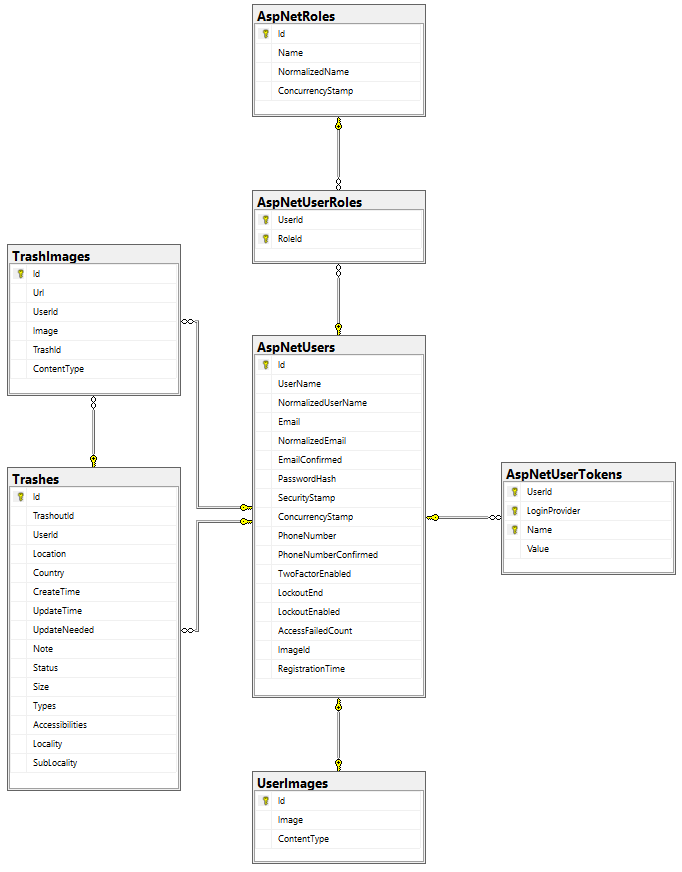
\includegraphics[width=0.7\linewidth]{database_sql}}
	\caption{Az adatbázis sémája leképzés előtt és után}
	\label{fig:database_scheme}
\end{figure}

\subsection{DTO-réteg}

A \texttt{TrashTracker.Data.DTOs} névtérben találhatóak az ún. DTO-k, magyarul adatátviteli osztályok. Ezeknek célja az adatbázisban található összes adat helyett csak az adott kontextusban szükséges adatokra való projektálás (pl. listanézet esetén nincs szükség a képekre, ezzel jelentős adatforgalmat megtakarítva). Emellett az egyes adatoknak itt vannak definiálva a validációs kritériumai és -hibaüzenetei (pl. a koordináták -180 és 180 között kell legyenek), ha azok bemeneti adatokként is szolgálnak, ellentétben nincs rá szükség, mivel feltehetjük, hogy a már adatbázisban szerepló adatok lekérdezéskor megfelelnek a megszorításoknak). Az adatátvitelhez használt objektumok az alábbiak:\\
\texttt{TrashTracker.Data.DTOs.In} (ki- és bemenő adatokhoz, validációkkal)
\begin{compactitem}
	\item \texttt{TokenFromGoogle}: a TrashOut-hoz való hozzáféréshez tartalmazza a tokent
	\item \texttt{TrashEdit}: egy bejelentett pont szerkeszthető tulajdonságait tartalmazza, melyből frissíthető egy \texttt{Trash} objektum
	\item \texttt{TrashFromTrashout}: egy TrashOut-ról letöltött pont adatait tartalmazza, melyből előállítható egy \texttt{Trash} objektum
	\item \texttt{TrashFromUser}: egy felhasználó által bejelentett pont adatait tartalmazza, melyből előállítható egy \texttt{Trash} objektum
	\item \texttt{UserEdit}: egy felhasználói profil szerkeszthető adatait tartalmazza, melyből frissíthető egy \texttt{TrashTrackerUser} objektum
	\item \texttt{UserLogin}: egy felhasználó bejelentkezéshez szükséges felhasználónév (vagy e-mail cím) és jelszó párosát tartalmazza
	\item \texttt{UserRegister}: egy felhasználó profil regisztráláshoz szükséges/megadható adatait tartalmazza, melyből előállítható egy \texttt{TrashTrackerUser} objektum
\end{compactitem}
\texttt{TrashTracker.Data.DTOs.Out} (kizárólag kimenő adatokhoz, validációk nélkül)
\begin{compactitem}
	\item \texttt{TrashDetails}: egy bejelentett pont adatlapján szereplő adatokat (azaz a képeket is) tartalmazza, mely egy \texttt{Trash} objektumból áll elő
	\item \texttt{TrashIndex}: egy bejelentett pont listanézetén szereplő adatokat tartalmazza, mely egy \texttt{Trash} objektumból áll elő
	\item \texttt{TrashMap}: egy bejelentett pont térképen levő koordinátái és szűrési tulajdonságait tartalmazza, mely egy \texttt{Trash} objektumból áll elő
	\item \texttt{TrashMapDetails}: egy bejelentett pont térképen levő adatlapján szereplő adatokat tartalmazza, mely egy \texttt{Trash} objektumból áll elő
	\item \texttt{UserDetails}: egy felhasználói profil oldalán szereplő adatokat tartalmazza, mely egy \texttt{TrashTrackerUser} objektumból áll elő
	\item \texttt{UserIndex}: egy felhasználói profil listanézetén szereplő adatokat tartalmazza, mely egy \texttt{TrashTrackerUser} objektumból áll elő
\end{compactitem}

\subsection{Vezérlő-réteg}

Ez a réteg felel minden beérkező kérés kiszolgálásáért, melyre több vezérlőosztály és a bennük található akció metódusok állnak rendelkezésre. Ezek az akciók általában a vezérlő és annak akciójából, illetve (ha van) paramétereiből összeállított "\texttt{/kontroller/akcio?param1=ertek1\&param2=ertek2}" formájú útvonalon érthetőek el.\\
Minden akcióhoz tartozik egy annotáció, mely megmondja mely HTTP-kérésre fussanak le. Ha egy akciót csak bizonyos szerepkörrel lehet elérni, akkor ahhoz is szerepel egy annotáció, mely megmondja melyik az a legalacsonyabb szerepkör, mellyel hozzáférhető az.\\
A kérés típusától független minden akció ad vissza valamilyen választ, mely lehet egy nézet, HTTP-állapotkód vagy egy JSON formátumú objektum, mely utóbbi a térképnek szolgáltatott adatokhoz szükséges.\\
Minden vezérlőt az ASP.NET Core keretrendszer példányosít, mely a HTTP-kérés beérkezésekor történik meg, mely példányon a megfelelő akciót futtatja le. A létrehozáshoz szükséges konstruktor paramétereit (pl. adatbázis-kontextus vagy felhasználó-kezelő) szintén ez a keretrendszer szolgáltatja ún. függőségi befecskendezéssel.\\
\texttt{HomeController}: A főoldal, azaz a térképen található adatok szolgáltatásáért felelős.
\begin{compactitem}
	\item \texttt{/OnMap}: az összes pont koordinátáit és szűrési tulajdonságait adja vissza \texttt{TrashMap} objektumokban
	\item \texttt{/OnMapDetails}: egy, a térképen való pontra kattintáskor megjelenő ablakban szereplő adatok adja vissza egy \texttt{TrashMapDetails} objektumban
\end{compactitem}
\texttt{TrashesController}: Az összes ponttal kapcsolatos, nem térképen megjelenő adatok nézeteinek szolgáltatásáért felelős
\begin{compactitem}
	\item \texttt{/Trashes?pageNumber=1\&pageSize=100\&searchString=abc\&showCleaned=false}: A pontok lapozható listanézetét adja vissza, melynek valamennyi paramétere opcionális. A paraméterek rendre az adott oldalszám, az oldal méret (hány pont legyen egy oldalon), a keresési szöveg, illetve a megtisztított pontok listázásának logikai értéke. Mivel a paraméterek opcionálisak, így ezek tetszőlegesen kihagyhatóak.
	\item \texttt{/Trashes/Details/id}: Egy ponthoz tartozó adatlapnak a nézetét adja vissza, ahol az \texttt{id} egy kötelező paraméter, mely meghatározza hányas sorszámú pontnak az adatlapja kerül visszaadásra.
	\item \texttt{/Trashes/Create}: GET kéréskor egy pont létrehozásához szükséges űrlap nézetét, POST kéréskor, benne az űrlap adataival pedig siker esetén egy átirányítást az előző oldalra, ellenben a GET kéréskor kapott űrlap nézetét a már kitöltött adatokat és hibaüzeneteit adja vissza.
	\item \texttt{/Trashes/Edit/id}: GET kéréskor egy pont módosításához szükséges űrlap nézetét, POST kéréskor, benne az űrlap adataival pedig siker esetén egy átirányítást az előző oldalra, ellenben a GET kéréskor kapott űrlap nézetét a már kitöltött adatokat és hibaüzeneteit adja vissza.
	\item \texttt{/Trashes/Delete/id}: GET kéréskor egy pont törléséhez tartózó megerősítő kérdés nézetét adja vissza, POST kéréskor pedig siker esetén átirányítást az előző oldalra.
\end{compactitem}
\texttt{UserController}: Az összes felhasználói fiókkal kapcsolatos, felhasználó-, bejelentkezés- és szerepkör-kezelésért felelős.
\begin{compactitem}
	\item \texttt{/User?pageNumber=1\&pageSize=100\&searchString=abc}: A felhasználói fiókok lapozható listanézetét adja vissza, melynek valamennyi paramétere opcionális. A paraméterek rendre az adott oldalszám, az oldal méret (hány fiók legyen egy oldalon), illetve a keresési szöveg. Mivel a paraméterek opcionálisak, így ezek tetszőlegesen kihagyhatóak.
	\item \texttt{/User/Details?userName=felhasznalo}: Egy felhasználói fiókhoz tartozó profiloldalnak a nézetét adja vissza, ahol az \texttt{userName} egy kötelező paraméter, mely meghatározza kinek a profilja kerül visszaadásra.
	\item \texttt{/User/Register}: GET kéréskor a fiók létrehozásához szükséges regisztrációs űrlap nézetét, POST kéréskor, benne az űrlap adataival pedig siker esetén egy átirányítást az főoldalra (illetve az új fiókba bejelentkezve), ellenben a GET kéréskor kapott űrlap nézetét a már kitöltött adatokat és hibaüzeneteit adja vissza.
	\item \texttt{/User/Login}: GET kéréskor a fiókba bejelentkezéshez szükséges űrlap nézetét, POST kéréskor, benne az űrlap adataival pedig siker esetén egy átirányítást az főoldalra (illetve a fiókba bejelentkezve), ellenben a GET kéréskor kapott űrlap nézetét a már kitöltött adatokat és hibaüzeneteit adja vissza.
	\item \texttt{/User/Delete/id}: GET kéréskor felhasználói fiók törléséhez tartózó megerősítő kérdés nézetét adja vissza, POST kéréskor pedig siker esetén átirányítást az előző oldalra.
\end{compactitem}

\subsection{Nézet-réteg}

Ez a réteg felel az egyes akciók által visszaadott nézetek definiálásáért. A \texttt{TrashTracker.Web.Views} névtérben található osztályok nem a C\# hagyományos szintaxisával, hanem a Razor-ével íródtak, mely tulajdonképpen egy \texttt{.html} formátumú fájl, benne C\# kódrészletekkel, ebből is adódik ezen fájlok kiterjesztésének a \texttt{.cshtml} neve.\\
Minden nézet kontrollerenként van csoportosítva, és minden nézetet visszaadó akciónak pontosan egy \texttt{.cshtml} formátumú nézetfájlja van. Ezek mellett a vannak ún. parciális nézetek is, melyek az egyes oldalakon szereplő, több helyen is ismétlődő tartalmat emelik ki külön fájlba, ezzel elkerülve az önismétlést. Ezen parciális nézetek fájljainak nevei az "\texttt{\_}" karakterrel kezdődnek, melyeknek többsége a Shared mappában található (pl. navigációs sáv, illetve az abban lévő fiók menüje).\\
\texttt{Home}
\begin{compactitem}
	\item \texttt{Index}: A főoldalon található térkép, illetve az ahhoz tartozó szűrési menüt tartalmazó nézet. A térkép viselkedése nem itt, hanem a \texttt{../../wwwroot/js/home.js} fájlban van definiálva, mivel a térképes megjelenítés dinamikája nem szerver-, hanem kilensoldalon történik a JavaScript nyelven íródott OpenLayers könyvtárcsomag segítségével.
\end{compactitem}
\texttt{Trashes}
\begin{compactitem}
	\item \texttt{Index}: A bejelentett pontok listanézetét megjelenítő nézet. Magát a listát az ebből az osztályból meghívott \texttt{\_IndexList} parciális nézet tartalmazza, ez csupán a szűrési menüt definiálja.
	\begin{compactitem}
		\item \texttt{\_IndexList}: A bejelentett pontok listanézetének a listáját tartalmazó parciális nézet, melynek tetején és alján található lapszámozás külön, \texttt{\_Pagination} nevű parciális nézetben kap helyet.
	\end{compactitem}
	\item \texttt{Details}: Egy bejelentett pont adatlapját megjelenítő nézet.
	\item \texttt{Create}: Egy pont bejelentésének űrlapját megjelenítő nézet.
	\item \texttt{Edit}: Egy bejelentett pont módosításának űrlapját megjelenítő nézet.
	\item \texttt{Delete}: Egy bejelentett pont törlését megerősítő üzenetét megjelenítő nézet.
\end{compactitem}
\texttt{User}
\begin{compactitem}
\item \texttt{Index}: A felhasználói fiókok listanézetét megjelenítő nézet. Magát a listát az ebből az osztályból meghívott \texttt{\_IndexList} parciális nézet tartalmazza.
\begin{compactitem}
	\item \texttt{\_IndexList}: A felhasználói fiókok listanézetének a listáját tartalmazó parciális nézet, melynek tetején és alján található lapszámozás külön, \texttt{\_Pagination} nevű parciális nézetben kap helyet.
\end{compactitem}
\item \texttt{Details}: Egy felhasználói fiók profiloldalát megjelenítő nézet, mely tartalmazza a \texttt{Trashes/\_IndexList} parciális nézetet, mely az adott fiók által bejelentett pontokat listázza.
\item \texttt{Login}: A bejelentkezési űrlapot megjelenítő nézet.
\item \texttt{Register}: A regisztrálási űrlapot megjelenítő nézet.
\item \texttt{Edit}: A profil szerkesztésének űrlapját megjelenítő nézet. Adminisztrátori fiókkal kiegészül az adott felhasználó szerepkörének módosításával.
\item \texttt{Delete}: Egy felhasználói fiók törlését megerősítő üzenetét megjelenítő nézet.
\end{compactitem}

\subsection{Kliensoldal}

Vannak olyan aloldalak (túlnyomó részben a főoldal/térkép), melyhez külön JavaScript nyelven írt kliensoldali programkódra is szükség van. Ezek a forráskódok a \texttt{TrashTracker.Web} projekt \texttt{wwwroot/js} könyvtárában találhatóak.\\
A \texttt{Home/Index} nézethez készült és hivatkozott \texttt{home.js} állomány tartalmazza magának a térkép objektumának a definícióját, illetve a szűrési menükben található gombok megnyomása esetén azt a függvényt, mely gombok állapota szerint változnak a térképen található pontok, melyek megfelelnek a feltételeknek. Emellett a pontra való kattintáskor megjelenő modális buborék is megjelenítésére szolgáló függvény is itt kap helyet.\\
A \texttt{Trashes/Index} nézet tetején található szűrési beállításokhoz készült a \texttt{index.js} segédprogram, mely segít az oldalra navigáláskor az adott szűrési feltételeket a hozzá megfelelő mezőbe beilleszteni.\\
A \texttt{Trashes/Create} és \texttt{Trashes/Edit} nézethez készült \texttt{position.js} fájl tartalmazza a "Jelenlegi hely meghatározása" gombra kattintáskor történő helymeghatározást, illetve annak megfelelő mezőibe való beillesztést.\\
Emellett a színséma alkalmazásáért és aloldalakon történő navigálások esetén való perzisztálásáért felel a \texttt{site.js} fájl, mely a közös, navigációs sávot is tartalmazó \texttt{Shared/\_Layout} nézetben van beszúrva, ezzel minden oldalon betöltésre kerül.

\section{Megvalósítás}

\section{Tesztelés}

\subsection{Tesztesetek}

\subsection{Fejlesztési lehetőségek}